\documentclass[9pt]{beamer}
%\PassOptionsToPackage[dvipsnames]{xcolor}
%\usepackage[dvipsnames]{xcolor}
\usepackage{tikz}
\usepackage{subfiles}
%\usepackage{subfig}
\usepackage{standalone}
\usepackage{graphicx} 
\usepackage{hyperref}
\usepackage{multimedia}
%\usepackage{subcaption}
\usepackage{subfig}
%\usepackage{amsmath}
%\usepackage{sfmath,sansmathaccent}
\usepackage{sansmathaccent}
%\pdfmapfile{+sansmathaccent.map}
%\usepackage{subcaption}
\usepackage{comment}


%%%%%%  listing

\usepackage{listings}
\usepackage{color}
\definecolor{codegreen}{rgb}{0,0.6,0}
\definecolor{codegray}{rgb}{0.5,0.5,0.5}
\definecolor{codepurple}{rgb}{0.58,0,0.82}
\definecolor{backcolour}{rgb}{0.95,0.95,0.92}
%Code listing style named "mystyle"
\lstdefinestyle{mystyle}
{
	backgroundcolor=\color{backcolour},   commentstyle=\color{codegreen},
	keywordstyle=\color{magenta},
	numberstyle=\tiny\color{codegray},
	stringstyle=\color{codepurple},
	basicstyle=\footnotesize,
	breakatwhitespace=false,         
	breaklines=true,                 
	captionpos=t,                    
	%   keepspaces=true,                 
	%numbers=false,                    
	%numbersep=5pt,                  
	showspaces=false,                
	showstringspaces=false,
	showtabs=false,                  
	tabsize=2
}
\lstset{style=mystyle}



%%%%%%%

\newcommand{\vect}[1]{\boldsymbol{#1}}
%\usepackage[table,xcdraw]{xcolor}  %to include tables with colors
\usepackage{pgfplots}
\pgfplotsset{compat=1.6}


\setbeamertemplate{footline}[page number]
\mode<presentation>{
%\usetheme{Malmoe}
%\usetheme{Antibes}
%\usetheme{warsaw}
\usetheme{Frankfurt}  %%
%\usetheme{Dresden}
%\usetheme{Madrid}
%\usetheme{Malmoe} %
%\usetheme{Ilmenau}
}
%\setbeamertemplate{footline}[\insertframenumber]

%\newcommand*\oldmacro{}%
%\let\oldmacro\insertshorttitle%
%\renewcommand*\insertshorttitle{%
% \oldmacro\hfill%
% \insertframenumber\,/\,\inserttotlaframenumber}

\AtBeginSection[]
{
\begin{frame}<beamer>
\frametitle{Plan}
\tableofcontents[currentsection]
\end{frame}
}


\definecolor{secinhead}{RGB}{249,196,95}
\definecolor{titlebg}{RGB}{51,51,51}
\definecolor{orangecl}{RGB}{255,81,0}

\setbeamercolor{secsubsec}{fg=secinhead,bg=black}
\setbeamercolor{frametitle}{fg=orangecl,bg=titlebg}\setbeamercolor{structure}{bg=titlebg,fg=orangecl}

\makeatletter
\let\insertsupervisor\relax
\newcommand\supervisortitle{Supervisor }
\makeatletter
\let\insertsupervisorinst\relax
\newcommand\supervisorinsttitle{Supervisorinst}
\mode<all>
{
  \newcommand\supervisor[1]{\def\insertsupervisor{#1}}
  \titlegraphic{}
}
\mode<all>
{
  \newcommand\supervisorinst[1]{\def\insertsupervisorinst{#1}}
  \titlegraphic{}
}
\defbeamertemplate*{title page}{supdefault}[1][]
{
  \vbox{}
  \vfill
  \begingroup
    \centering
		\begin{columns}  
		\column{0.33\textwidth}
		 \includegraphics[width=0.5\linewidth]{images/ECN.png}
		 \column{0.33\textwidth}
		 \begin{center}
		 \includegraphics[width=0.5\linewidth]{images/ArcelorMittal_logo.png}
		 \end{center}
	     \column{0.33\textwidth}
	     \begin{flushright}
		 \includegraphics[width=0.5\linewidth]{images/Uni-logo.png}
		 \end{flushright}
		 \end{columns}
    \vskip1em\par
    \begin{beamercolorbox}[sep=8pt,center,#1]{title}
%      \usebeamerfont{title}
      \inserttitle\par%
      \ifx\insertsubtitle\@empty\relax%
      \else%
        \vskip0.25em%
        {%\usebeamerfont{subtitle}
        \usebeamercolor[fg]{subtitle}\insertsubtitle\par}%
      \fi%     
    \end{beamercolorbox}%
    \vskip1em\par
    \begin{beamercolorbox}[sep=8pt,center,#1]{author}
    Presented By:\\
%      \usebeamerfont{author}
      \textbf{\insertauthor} \\
%      \usebeamerfont{institute}
      \insertinstitute
    \end{beamercolorbox}
   %     \begin{beamercolorbox}{institute}
   %   \usebeamerfont{institute}\insertinstitute
   % \end{beamercolorbox}
    \ifx\insertsupervisor\relax\relax\else
    \begin{beamercolorbox}[sep=8pt,center,#1]{author}
%      \usebeamerfont{author}
      \supervisortitle: \\ \textbf{~\insertsupervisor} \\
%      \usebeamerfont{institute}
      \insertsupervisorinst
    \end{beamercolorbox}\fi
    %\begin{beamercolorbox}[sep=8pt,center,#1]{institute}
    %  \usebeamerfont{institute}\insertinstitute
    %\end{beamercolorbox}
    \begin{beamercolorbox}[sep=8pt,center,#1]{date}
%      \usebeamerfont{date}
      \insertdate
    \end{beamercolorbox}\vskip0.5em
    {\usebeamercolor[fg]{titlegraphic}\inserttitlegraphic\par}
  \endgroup
  \vfill
  
}
\setbeamertemplate{title page}[supdefault][colsep=-4bp,rounded=true,shadow=\beamer@themerounded@shadow]\makeatother

\title{Finite Element Simulation of 2D Metal Strip Vibration in
Hot-Dip Galvanization Process}
%\subtitle{Reissner Mindlin Plate}
\author{Emayavaramban ELANGO}
\supervisor{PHAM Van Thang}
\supervisorinst{PHAM Van Thang }
\institute{\'Ecole centrale De Nantes}

\supervisorinst{ArcelorMittal Maizi\`eres Research SA}
%\supervisorinst{\textbf{ArcelorMittal} Maizi\`eres Research SA }
\date{\today}


\begin{document}
%\begin{frame}

\frame{\titlepage}


\begin{frame}
\frametitle{Table of Content}
\tableofcontents
\end{frame}
\section{Introduction}

\begin{frame}
\frametitle{Objective of the Internship}
\begin{itemize}
\item To understand the Hot-dip galvanization process and to have an idea about the loads and boundary condition.
\item To find existing research about finite element of strip used in this process.
\item To formulate plate equation of motion
\item To code accurate and efficient finite element program from scratch
\item To test the finite element code with analytical and existing numerical methods
\item To find a way to integrate with existing control algorithms.
 


\end{itemize}

\end{frame}


\subsection{ArcelorMittal Maizi\`eres research SA}
\begin{frame}{ArcelorMittal Maizi\`eres research SA}
\begin{itemize}
\item ArcelorMittal is the global leader in steel production and mining activity.
\item Formed in 2006 by merging MittalSteel and Arcelor.The headquarters is in Luxembourg.
\item ArcelorMittal spends hundreds of millions of dollars in research and development.
\item ArcelorMittal Maizi\`eres research SA is the research center where this thesis is undertaken under the department of measurement and control.
\item The main task of this department was to explore and fine turn the new measurement techniques in profit of increasing the quality of the steel production. 
\item The control team of the department is specialized in developing advanced control strategies (Model Predictive control, Model - based control etc,.) to continuously improve the comfort of operators and the product quality.


\end{itemize}

\end{frame}



\subsection{Hot-Dip Galvanization Process}
\begin{comment}
\begin{frame}
\begin{columns}
\column{0.6\textwidth}
\begin{figure}
\centering
%\subfloat[Schematics of the Hot-Dip Galvanization Line \label{fig:galvline}]
\subfloat[\captionformat{labelformat=empty}]{\includestandalone[mode=image,build={quote={}},width=0.88\textwidth]{"tikz/GalvLine"}} \quad
\end{figure}
\column{0.4\textwidth}
\includegraphics[width=1\textwidth]{images/galv_line.jpg}
%\includegraphics[scale=1]{images/galv_line.png}
\end{columns}
\end{frame}
\end{comment}

%\begin{comment}
\begin{frame}
\frametitle{Hot-Dip Galvanization Process}
\begin{figure}
\centering
\subfloat{\includestandalone[mode=image,build={quote={}},width=11.5cm]{"tikz/GalvLine_ppt"}} 
\caption{Schematics of the Hot-Dip Galvanization Line}
\end{figure}
\end{frame}




\begin{frame}
\begin{columns}
\column{0.65\textwidth}
\begin{figure}

\centering
\subfloat{\includestandalone[mode=image,build={quote={}},width=7.5cm]{"tikz/GalvLine_Real"}} 
\caption{Hot-Dip Galvanization Line}
\end{figure}
\column{0.35\textwidth}
\begin{itemize}
\item A thin layer of Zinc is coated to increase the corrosion resistance of steel
\item Air knives control the thickness of the Zinc layer
\item Excessive vibration results in uneven coating.
\item Electromagnets are used to control the  vibration of the strip. 
\end{itemize}
\end{columns}
\end{frame}
%\end{comment}


\section{Axially Moving Plate}
\begin{frame}\frametitle{Axially Moving Plate}
%\begin{columns}
%\column{0.6\textwidth}

\begin{figure}[ht!]
\centering\includestandalone[mode=image,build={quote={}},width=7.5cm]{"tikz/domain"}
\caption{Description of domain}
\label{fig:Domain}
\end{figure}
%\column{0.4\textwidth}
\begin{itemize}

\item $\Omega$ is the two dimensional domain strictly in xy plane 
\item $h$ is the thickness of the plate 
\item $\Omega_1$...$\Omega_i$ are the sub-domains where pressure forces $q_1$..$q_i$ are applied
\item $V$ is the line speed and  $N_y$ is the tension on the line
\item $L$ is the length and  $B$ is the width 

\end{itemize}



%\end{columns}

\end{frame}

\subsection{Hamilton Principle}


\begin{frame}\frametitle{Hamilton Principle}

The modified form of the Hamilton principle is taken as.

 \begin{equation}\label{eq:HAM_P}
 \delta H=\int_{t_0}^{t_1} \left( \delta U - \delta K + \delta W + \delta M \right) dt  = 0  
 \end{equation}
 \begin{equation}\label{eq:HAM_P_C}
  \delta \mathbf{u} \Big|_{t_0}^{t_1} = 0
 \end{equation}
 $\delta$ is the variation, $t_0$ and $t_1$ are any arbitrary temporal points, $U$ is the total potential energy , $K$ is the kinematic energy and $W$ is the work performed by external forces on the system. $\mathbf{u}$ is the total displacement of the plate. $M$ is the momentum transports at boundaries y=0 and y = L. 
 \begin{equation}\label{eq:vr_M}
\delta M= \int_{0}^{W} \int_{-h/2}^{h/2}L \rho \mathbf{v} \delta \mathbf{u} \Big|_{y=0}^{y=L} dz dx  = 0
 \end{equation}
Here, $\mathbf{v}$ is the total velocity vector of the plate. $M$ becomes zero because the line speed is equal at the boundaries. So, there is no overall change in the mass of the plate.
\end{frame}

\subsection{Plate Theories}
\begin{frame}
\frametitle{Plate Theories}

\begin{block}{Plate assumptions}
\begin{itemize}
\item The plate thickness does not change after deformation.  $\epsilon_{zz} = 0$ 

\item  In the absence of axial deformation, any point in the mid-plane only moves either in an upward or downward direction

\item  The flat planes normal to mid-plane will always be a flat planes, they won't distort. 
\end{itemize}
\end{block}
\begin{columns}
\column{0.65\textwidth}
\begin{figure}[ht!]
\centering\includestandalone[mode=image,build={quote={}},width=7cm]{"tikz/Plate_Theory"}
%\caption{Description of domain}
\label{fig:Domain}
\end{figure}
\column{0.35\textwidth}
\begin{block}{Plate displacement}
\begin{equation*}
 \begin{split}
\tilde{\mathbf{u}} =
\left\{
\begin{array}{r}
 - z \theta_x \left(x,y\right) \\
 - z \theta_y \left(x,y\right)\\
  w \left(x, y \right) 
\end{array} \right\}
\end{split}
\end{equation*}
\end{block}

\end{columns}
\end{frame}

\begin{frame}
\begin{block}{Kirchhoff Plate}
 Kirchhoff plate theory is well suitable for thin plates. A straight line normal to mid-plane stays normal and straight after deformation($\phi_x=0$).  Because of this assumption, the shear strains ($\epsilon_{23}$ and $ \epsilon_{13}$)  are neglected.


\begin{align*}
\theta_x  = \frac{\partial w }{\partial x}  \quad & \quad
\theta_y  = \frac{\partial w }{\partial y} 
\end{align*}

\end{block}

\begin{block}{Reissner Mindlin plate theory}
The Reissner Mindlin plate theory is developed for the thick plates but can be used for thin plates with caution.  For Reissner Mindlin plate theory, the line normal to the middle plate will not necessarily be normal after deformation, but will be straight. $\phi_x$ and $\phi_y$ are the angles between plane normal to middle plane and plane of actual deformation.  

\begin{align*}\label{eq:thetaRM}
\theta_x  = \frac{\partial w }{\partial x} + \phi_x \quad & \quad
\theta_y  = \frac{\partial w }{\partial y} + \phi_y
\end{align*}
\end{block}
\end{frame}

\begin{frame}\frametitle{Potential Energy}
The total potential strain energy $U$ is given as.

\begin{equation*}
U=\frac{1}{2} \int\int\int_\Gamma \left(\vect{\epsilon}\right)^T \vect{\sigma} d \Gamma 
=
\frac{1}{2} \int\int\int_\Gamma \left(\vect{\epsilon}^B\right)^T \vect{\sigma}^B + \left(\vect{\epsilon}^S\right)^T \vect{\sigma}^S + \left(\vect{\epsilon}^A\right)^T \vect{\sigma}^A d \Gamma
\end{equation*}
B,S,A on the superscript indicates bending, shear and axial components of the strain and stress. Using strain formula each of the strain is.

\begin{align*}
\vect{\epsilon}^B = -z
\begin{bmatrix}
\dfrac{\partial w^2 }{\partial x^2}
\\
\dfrac{\partial w^2 }{\partial y^2}
\\
\dfrac{\partial w^2 }{\partial x \partial y}
\end{bmatrix}
=
 z \boldsymbol{\kappa}
\qquad
\vect{\epsilon}^S = \dfrac{1}{2}
\begin{bmatrix}
\dfrac{\partial w}{\partial x}-\theta_x 
\\
\dfrac{\partial w}{\partial y}-\theta_y 
\end{bmatrix}
\qquad
\vect{\epsilon}^A = 
 \left( \dfrac{\partial w}{\partial y} \right)^2
 =
 \left( w_{,2} \right)^2
\end{align*}

\begin{columns}
\column{0.5\textwidth}
For Kirchhoff Plate
\begin{equation*}
\vect{\epsilon}^S =
\begin{bmatrix}
0
\\
0
\end{bmatrix}
\end{equation*}



\column{0.5\textwidth}
For Reissner Mindlin Plate
\begin{equation*}
\vect{\epsilon}^S = \dfrac{1}{2}
\begin{bmatrix}
-\phi_x
\\
-\phi_y
\end{bmatrix}
\end{equation*}
\end{columns}
\end{frame}

\begin{frame}

The Hooke's law for the  homogenous linear isotropic material is considered.

\begin{equation*}
\vect{\sigma}^B = \begin{bmatrix}
\sigma_{11}
\\
\sigma_{22}
\\
 \sigma_{12}
\end{bmatrix}
=\dfrac{1}{1-\nu^2}
\begin{bmatrix}
E & \nu E & 0
\\
\nu E & E & 0
\\
0 & 0 & (1-\nu^2)G
\end{bmatrix}
\begin{bmatrix}
\epsilon_{11}
\\
\epsilon_{22}
\\
 \epsilon_{12}
\end{bmatrix}
=
\vect{D}
\vect{ \epsilon}^B
\end{equation*}


\begin{align*}
\vect{\sigma}^S = \begin{bmatrix}
\sigma_{31}
\\
 \sigma_{32}
\end{bmatrix}
=KG
\begin{bmatrix}
1 & 0 
\\
0 & 1 
\end{bmatrix}
\begin{bmatrix}
\epsilon_{31}
\\
\epsilon_{32}
\end{bmatrix}
=
\vect{D_c} \vect{\epsilon}^S
\qquad
\qquad
\vect{\sigma}^A = \begin{bmatrix}
\sigma_{22}
\end{bmatrix}
=
\begin{bmatrix}
N_y
\end{bmatrix}
\end{align*}



$E$ is Young's modulus, $\nu$ is the Poisson's ratio and $G$ is the shear modulus which is given by $G=E / 2 ( 1+\nu ) $. $K$ is the shear correction factor. Shear correction factor value of 5/6 is used for this application. Substituting everything in strain energy formula and taking variation gives. 
\begin{equation*}. 
U=\frac{1}{2} \int\int_\Omega \left[ \int_{-h/2}^{+h/2} z^2 dz\right] \vect{\kappa}^T {\vect{D}} \vect{\kappa} 
+ \left[ \int_{-h/2}^{+h/2} dz\right]
(
\left(\vect{\epsilon}^S
\right)^T {\vect{D_c}} \vect{\epsilon}^S 
+ 
 \left(\vect{\epsilon}^A\right)^T \vect{\sigma}^A 
 ) d \Omega
\end{equation*}


\begin{equation*}
\delta U=\int\int_\Omega 
\vect{\kappa}^T \vect{\tilde{D}} \delta\vect{\kappa} 
+ 
\left(\vect{\epsilon}^S\right)^T \vect{\tilde{D_c}} \delta \vect{\epsilon}^S 
+ 
w_{,2}\tilde{\vect{\sigma}^A} \delta w_{,2} d \Omega
\end{equation*}

\end{frame}
\begin{frame}\frametitle{Kinetic Energy}
Based on Euler - Lagrange formulation the velocity is given as
\begin{equation*}\label{eq:v}
  \mathbf{v}=\left\{ \dot{u_1}+V_2u_{1,2} \quad  \dot{u_2}+V_2u_{2,2} \quad  \dot{u_3}+V_2u_{3,2} \right\}^T
\end{equation*}
The kinetic energy is 
\begin{equation*}\label{eq:KE}
K = \frac{1}{2} \int \int \int_{\Gamma} \mathbf{v}^T\rho\mathbf{v} d\Gamma
=\frac{1}{2} 
\int \int_\Omega \int_{-\frac{h}{2}}^{\frac{h}{2}} 
\rho \vect{ \dot{u}} ^T    \vect{ \dot{u}}
+
2 \rho  V_2 \vect{ \dot{u}} ^T   \vect{u}_{,2}
+
\rho  V_2^2  (\vect{u}_{,2})^T   \vect{u}_{,2}
\quad
 dz 
 d\Omega
\end{equation*}

\begin{equation*}
K=\frac{1}{2} 
\int \int_\Omega
\rho  \vect{\dot{\tilde{u}}}^T  \vect{Z}    \vect{\dot{\tilde{u}}}
+
2 \rho  V_2 \vect{\dot{\tilde{u}}}^T  \vect{Z}     \vect{\tilde{u}}_{,2}
+
\rho  V_2^2 (\vect{\tilde{u}}_{,2})^T   \vect{Z}      \vect{\tilde{u}}_{,2}
\quad
 d\Omega
\end{equation*}

\begin{equation*}
 \vect{Z}  = 
 \begin{bmatrix}
h   &  0 & 0 \\
0   &  \frac{h^3}{12}& 0 \\
0   &  0 & \frac{h^3}{12} \\
\end{bmatrix}
\qquad
(and)
\qquad
 \vect{\tilde{u}}  = 
 \begin{bmatrix}
w   \\
\theta_x    \\
\theta_y   \\
\end{bmatrix}
\end{equation*}

Finally the variation of the kinetic energy
\begin{equation*}\label{eq:vr_KE}
\delta K
= 
\int \int_\Omega
\rho  \vect{\dot{\tilde{u}}}^T  \vect{Z}    \delta \vect{\dot{\tilde{u}}}
+
\rho  V_2 \delta \vect{\dot{\tilde{u}}}^T  \vect{Z}      \vect{\tilde{u}}_{,2}
+
\rho  V_2 \vect{\dot{\tilde{u}}}^T  \vect{Z}     \delta \vect{\tilde{u}}_{,2}
+ 
\rho  V_2^2 (\vect{\tilde{u}}_{,2})^T   \vect{Z}      \delta \vect{\tilde{u}}_{,2}
\quad
 d\Omega
\end{equation*}

\end{frame}


\subsection{Final Weak Form}
\begin{frame}\frametitle{Final Weak form}



The Transverse distributed forces $q_j$ is applied in the regions in $\Omega^j$ is given as
\begin{equation*}\label{eq:vr_W}
\delta W=\sum_j^{nb} \int_{\Omega^j} q_j \delta \vect{\tilde{u}} \quad  d \Omega^j
\end{equation*}


Substituting everything in the Hamilton principle and taking integration by parts gives the final weak form of the axially moving and axially tensed plate.
%\begin{equation}
%\begin{split}
% \int \int_\Omega 
%\rho \dot{\tilde{u_i}} Z_{ij} \delta \tilde{u_i}
%+
%\rho V_1 \delta {\tilde{u_i}} Z_{ij} \tilde{u}_{j,1} 
%+  
%\rho V_1 {\tilde{u_i}} Z_{ij} \delta \tilde{u}_{j,1}  
% d \Omega  \Big|_{t_0}^{t_1} 
% \\ +
% \int_{t_0}^{t_1} \int \int_\Omega 
%-
%\rho \ddot{\tilde{u_i}} Z_{ij} \delta {\tilde{u_j}}
%-
%\rho V_1 \delta {\tilde{u_i}} Z_{ij} \dot{\tilde{u}}_{j,1} 
%-  
%\rho V_1  \tilde{u_i} Z_{ij} \delta \dot{\tilde{u}}_{j,1} 
%+
%\rho V_1^2 \tilde{u}_{i,1} Z_{ij} \delta \tilde{u}_{j,1}
%\\ 
%- 
%\kappa^T \tilde{D} \delta\kappa 
%-
%\left(\epsilon^S\right)^T \tilde{D_c} \delta\epsilon^S 
%- 
% w_{, \alpha} \tilde{\sigma}^A  \delta w_{, \alpha}  d \Omega     
% +   
%\sum_j^{nb} \int_{\Omega_j} q_j \delta \tilde{u}_i  d \Omega_j dt = 0
%\end{split} 
%\end{equation}



\begin{equation*}
\begin{split}
\int \int_\Omega 
\rho \vect{\ddot{\tilde{u}}}^T \vect{Z} \delta \vect {{\tilde{u}}}
+  
\rho V_1 \delta \vect{\tilde{u}} \vect{Z} \vect{\dot{\tilde{u}}}_{,2} 
+ 
\rho V_1  \vect{\tilde{u}} \vect{Z} \delta \vect{\dot{\tilde{u}}}_{,2} 
-
\rho V_1^2 \vect{\tilde{u}}_{,2} \vect{Z} \delta \vect{\tilde{u}}_{,2}
\\ 
+ 
\vect{\kappa}^T \vect{\tilde{D}} \delta \vect{\kappa} 
+
\left(\vect{\epsilon}^S\right)^T \vect{\tilde{D_c}} \delta\vect{\epsilon}^S 
+
 w_{, 2} \vect{\tilde{\sigma}}^A  \delta w_{, 2}  d \Omega     
 =  
\sum_j^{nb} \int_{\Omega^j} q_j \delta \vect{\tilde{u}}  d \Omega^j 
\end{split} 
\end{equation*}

First term in the equation corresponds to the local acceleration. second and third terms are the Coriolis acceleration and the fourth term is the centripetal acceleration.

\end{frame}



\section{Finite Element Formulation}
\begin{frame}\frametitle{Finite Element Formulation}
\begin{figure}[h]
\centering
\includestandalone[mode=image,build={quote={}},width=7.5cm]{"tikz/FEMdomain"}
%\caption{NAS277} \label{NAS277sch}
\caption{FEM domain}
\label{fig:fem_domain}
\end{figure}


The description of the domain is given in the the figure.\ref{fig:fem_domain}.  $\Omega$ is the total two dimensional domain in the x , y plane. The domain is discretized into small elements $\Omega^e$. $\Omega^1 \cdots \Omega^n$ are the regions where transverse distributed loads $(q_1 \cdots q_i)$ are described. $\partial \Omega$ is the boundary of the domain. $\partial \Omega _ d$ is part of the boundary where Dirichlet boundary condition is applied. 


\end{frame}

\begin{frame}
The Displacement field of the each element is the function of displacement of degree of freedom of each  node, which lets us have a finite number of unknowns to denote the over all displacement field of the domain. 

Since it is a plate element, three independent degrees of freedom are described for each node. 
\begin{equation*}
\begin{split}
\tilde{\mathbf{u}} = \left[ w, \theta_x , \theta_y  \right]^T
\end{split}
\end{equation*}
$w$ represents the transverse displacement. $\theta_x$ and $\theta_y$ represents the rotations. 
\begin{equation}
\theta_x =\frac{\partial w}{\partial x} \qquad
 \theta_y  =\frac{\partial w}{\partial y}
\end{equation}
The approximate displacement of the element is the given as sum of product of nodal degree of freedom and its corresponding shape functions ($N$,$\overline{N}$,$\overline{\overline{N}}$).
\begin{equation}\label{eq:approx_disp}
\begin{split}
\tilde{\mathbf{u}} \approx \sum_{i=1}^{n}\left(N_iw_i+\overline{N}_i\theta_{x_i} +\overline{\overline{N}}_i\theta_{y_i}\right)
\end{split}
\end{equation}

\end{frame}


\begin{comment}
\begin{frame}\frametitle{Finite Element Formulation}
matrix from

\end{frame}

\subsection{Reissner Mindlin Plate Element (QUAD4)}
\begin{frame}\frametitle{Reissner Mindlin Plate Element (QUAD4)}

The displacement field over the element is given as the sum of product of shape function and nodal displacements. Here $n$ is the total number of nodes in an element

 \begin{columns}
 \column{0.6\textwidth}
\begin{block}{Displacement field of an element}
 \begin{equation*}
\begin{split}
\tilde{\mathbf{u}} \approx \sum_{i=1}^{n}\left(N_iw_i+\overline{N}_i\theta_{x_i} +\overline{\overline{N}}_i\theta_{y_i}\right)
\end{split}
\end{equation*}
\begin{equation*}
\begin{split}
\tilde{u} = \left[ w, \theta_x , \theta_y  \right]^T
\theta_x =\frac{\partial w}{\partial x}
 \theta_y  =\frac{\partial w}{\partial y}
\end{split}
\end{equation*}
\end{block}
 \column{0.4\textwidth}
%
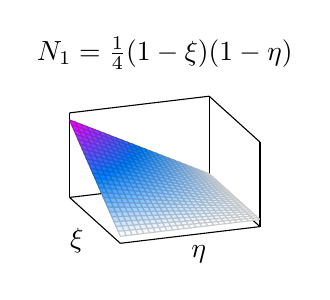
\begin{tikzpicture}
\pgfplotsset{compat=1.8,width=4cm,compat=newest}
  \begin{axis}[colormap/cool,
  title = {$N_1=\frac{1}{4}(1-\xi)(1-\eta)$},
  ticks=none,
  %axis x line*=box,axis y line*=box, 
  %axis z line=none, 
  				view/h=70,	
  				%,hide axis
  				%axis on top,
				%axis lines*=box, 
				  	 ,xlabel = $\xi$
     , ylabel = $\eta$, 				
  				]
    \addplot3[surf,
	domain=-1:1,
	domain y=-1:1,    
    ] {0.25*(1 - x - y + x*y)};
  \end{axis}
\end{tikzpicture}

\end{columns}


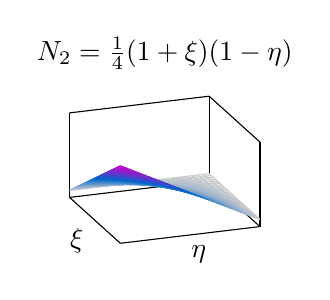
\begin{tikzpicture}
\pgfplotsset{compat=1.8,width=4cm,compat=newest}
  \begin{axis}[colormap/cool,
  	%hide axis,
  	view/h=70,
  	ticks=none,
  	title = { $N_2=\frac{1}{4}(1+\xi)(1-\eta)$ },
  	 xlabel = $\xi$
     , ylabel = $\eta$,
     axis lines*=box, 
  	]
    \addplot3[surf,
	domain=-1:1,
	domain y=-1:1,    
    ]  {0.25*(1 + x - y - x*y)};
  \end{axis}
 
  
\end{tikzpicture}
~
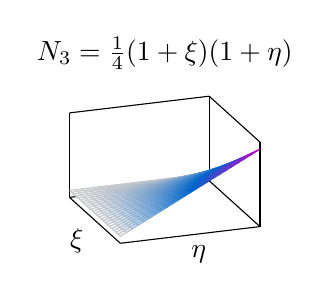
\begin{tikzpicture}
\pgfplotsset{compat=1.8,width=4cm,compat=newest}
  \begin{axis}[colormap/cool,
  %,hide axis
  view/h=70,
  ticks=none,
  title = { $N_3=\frac{1}{4}(1+\xi)(1+\eta)$ },
    	 xlabel = $\xi$
     , ylabel = $\eta$
  ,axis lines*=box,
   ]
    \addplot3[surf,
	domain=-1:1,
	domain y=-1:1,    
    ]  {0.25*(1 + x + y + x*y)};
  \end{axis}
\end{tikzpicture}
~
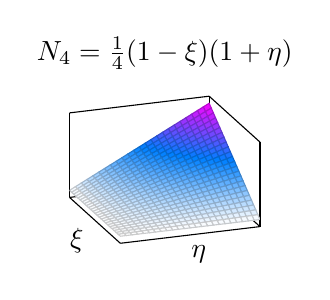
\begin{tikzpicture}
\pgfplotsset{compat=1.8,width=4cm,compat=newest}
  \begin{axis}[colormap/cool,
  %,hide axis,
  view/h=70,
  ticks=none,
  title = { $N_4=\frac{1}{4}(1-\xi)(1+\eta)$ },
    	 xlabel = $\xi$
     , ylabel = $\eta$
    ,axis lines*=box,
  ]
    \addplot3[surf,
	domain=-1:1,
	domain y=-1:1,    
    ]  {0.25*(1 - x + y - x*y)};
  \end{axis}
\end{tikzpicture}



\end{frame}
\end{comment}

\subsection{Reissner Mindlin plate element (QUAD4)}
\begin{frame}\frametitle{Reissner Mindlin Plate Element (QUAD4)}

\begin{columns}
\column{0.6\textwidth}
\begin{figure}[h!]
\centering

\includestandalone[mode=image,build={quote={}},width=1\textwidth]{"tikz/iso"}
\caption{Jacobian transformation} 
\label{fig:JacTrans_quad}
\end{figure}
\column{0.4\textwidth}




 
\begin{equation*}\label{eq:MITC4_SF}
\begin{split}
N_1  =\frac{1}{4}(1-\xi)(1 -\eta)
\\
N_2=\frac{1}{4}(1+\xi)(1-\eta) 
 \\
N_3  =\frac{1}{4}(1+\xi)(1+ \eta)
 \\
N_4 =\frac{1}{4}(1-\xi)(1+\eta)\end{split}
\end{equation*}
\end{columns}

\begin{equation}
\left\{
\begin{array}{r}
\dfrac{\partial N }{ \partial \xi }  \\
\dfrac{\partial N }{ \partial \eta }  \\
\end{array}
\right\}
=
\begin{bmatrix}
\dfrac{ \partial x }{\partial \xi }   &
\dfrac{ \partial y }{\partial \xi } \\
\dfrac{ \partial x }{\partial \eta }   &
\dfrac{ \partial y }{\partial \eta } \\
\end{bmatrix}
\left\{
\begin{array}{r}
\dfrac{\partial N }{ \partial x }  \\
\dfrac{\partial N }{ \partial y }  \\
\end{array}
\right\}
\quad
J=\begin{bmatrix}
\dfrac{ \partial x }{\partial \xi }   &
\dfrac{ \partial y }{\partial \xi } \\
\dfrac{ \partial x }{\partial \eta }   &
\dfrac{ \partial y }{\partial \eta } \\
\end{bmatrix}
\end{equation}



\end{frame}

\begin{comment}



\begin{frame}
\frametitle{Representation of Displacements and Strains in terms of Shape Function.}
The FE approximation 
\begin{equation*}
\tilde{\mathbf{u}} \approx \sum_{i=1}^{n}\left(N_iw_i+\overline{N}_i\theta_{x_i}+\overline{\overline{N}}_i\theta_{y_i}\right)
\end{equation*}
is written in matrix format as
\begin{equation*}
\tilde{\mathbf{u}} \approx 
\begin{bmatrix}
N_1 & 0 & 0  & \cdots & N_{nN} & 0 & 0 \\
0 & \overline{N}_1 & 0  & \cdots & 0 & \overline{N}_{nN} & 0 \\
0 & 0 & \overline{\overline{N}}_1 & \cdots & 0 & 0 & \overline{\overline{N}}_{nN} \\
\end{bmatrix}
\left\{
\begin{array}{r}
w_1 \\
\theta_{x_1} \\
\theta_{y_1} \\
\vdots \\
w_{nN} \\
\theta_{x_{nN}} \\
\theta_{y_{nN}} \\
\end{array} \right\}
=
\mathbf{N} \tilde{\mathbf{u}}^e 
\end{equation*}
Similarly other terms of the Finite Element Matrices are
%\begin{equation*}
\begin{align*}
\dot{\tilde{ \mathbf{ u}} } & \approx  \mathbf{N}  \dot{\tilde{\mathbf{u}}}^e
&  
\ddot{\tilde{ \mathbf{ u}} } &  \approx   \mathbf{N}  \ddot{\tilde{\mathbf{u}}}^e
&
\mathbf{ \kappa } & \approx   \mathbf{ B } \tilde{\mathbf{u}}^e
&
\tilde{\mathbf{\epsilon}}^S  & \approx  \mathbf{ B_S }\tilde{\mathbf{u}}^e
\\
\tilde{u}_{1, \alpha}  & \approx  \mathbf{ H_A }\tilde{\mathbf{u}}^e
&
\tilde{u}_{\alpha, 1}  & \approx  \mathbf{ H_v }\tilde{\mathbf{u}}^e
&
\tilde{w}  & \approx  \mathbf{ N_f }\tilde{\mathbf{u}}^e
\end{align*}
%\end{equation*}
\end{frame}
\end{comment}

\subsection{Kirchhoff Plate Element (PAT)}
\begin{frame}\frametitle{Kirchhoff Plate Element (PAT)}

The triangle element with three nodes, is given here.

\begin{equation*}
N = 
\begin{bmatrix}
                 P(1)-P(4)+P(6)+2*(P(7)-P(9))\\
                 -b(2)*(P(9)-P(6))-b(3)*P(7)\\
                 -c(2)*(P(9)-P(6))-c(3)*P(7)\\
                 P(2)-P(5)+P(4)+2*(P(8)-P(7))\\
                 -b(3)*(P(7)-P(4))-b(1)*P(8)\\
                 -c(3)*(P(7)-P(4))-c(1)*P(8)\\
                 P(3)-P(6)+P(5)+2*(P(9)-P(8))\\
                -b(1)*(P(8)-P(5))-b(2)*P(9)\\
                -c(1)*(P(8)-P(5))-c(2)*P(9)\\
\end{bmatrix}
\end{equation*}

 The element is based on a polynomial expression of nine terms.
 

\begin{equation*}\label{eq:poly}
\begin{split}
\textbf{P} & = [
\begin{matrix}
L_1
&
L_2
&
L_3
&
L_1 L_2
&
L_2 L_3
&
L_3 L_1
\end{matrix} \\
& \quad
\begin{matrix}
L_1^2L_2+\frac{1}{2}L_1L_2L_3(3(1-\mu_3)L_1-(1+3\mu_3)L_2+(1+3\mu_3)L_3) )
\end{matrix}\\
& \quad
\begin{matrix}
L_2^2L_3+\frac{1}{2}L_1L_2L_3(3(1-\mu_1)L_2-(1+3\mu_1)L_3+(1+3\mu_1)L_1) )
\end{matrix}\\
& \quad
\begin{matrix}
L_3^2L_1+\frac{1}{2}L_1L_2L_3(3(1-\mu_2)L_3-(1+3\mu_2)L_1+(1+3\mu_2)L_2) )
\end{matrix} ]
\end{split}
\end{equation*}


\end{frame}

\begin{frame}\frametitle{Area coordinate}

\begin{columns}
\column{0.8\textwidth}

\begin{figure}[h!]
\centering

\includestandalone[mode=image,build={quote={}},width=1\textwidth]{"tikz/area_cod"}
\caption{Area coordinate} 
\label{fig:areacord}
\end{figure}

\end{columns}

\begin{equation*}
L_1 = \frac{A_1}{A} \quad L_2 = \frac{A_2}{A} \quad L_3 = \frac{A_3}{A}
\end{equation*}
\begin{equation*}
L_1 + L_2 + L_3 = 1
\end{equation*}
\begin{equation*}
\left\{
\begin{array}{r}
 \frac{\partial}{\partial x}\\
\frac{\partial}{\partial y}
\end{array} \right\}
=
\frac{1}{4 A}
\begin{bmatrix}
y_2-y_3 & y_3-y_1 & y_1-y_2 \\
x_2-x_3 & x_3-x_1 & x_1-x_2
\end{bmatrix} 
\left\{
\begin{array}{r}
 \frac{\partial}{\partial L_1}\\
 \frac{\partial}{\partial L_2}\\
 \frac{\partial}{\partial L_3}
\end{array} \right\}
\end{equation*}
\end{frame}

\begin{comment}
\begin{frame}


\begin{equation*}
\tilde{\mathbf{u}}  \approx 
\left\{
\begin{array}{r}
w \\
\theta_x \\
\theta_y \\
\end{array} \right\}
=
\begin{bmatrix}
{N}_{1} & N_{2} & N_{3} &{N}_{4} &\cdots & N_{9} \\
{N}_{1,1} & N_{2,1} & N_{3,1} &{N}_{4,1} &\cdots & N_{9,1} \\
{N}_{1,2} & N_{2,2} & N_{3,2} &{N}_{4,2} &\cdots & N_{9,2} 
\end{bmatrix} 
\left\{
\begin{array}{r}
w_1 \\
\theta_{x_1} \\
\theta_{y_1} \\
w_2 \\
\vdots \\
\theta_{y_{3}} \\
\end{array} \right\}
=
\mathbf{N} \mathbf{\tilde{u}^e} 
\end{equation*}
the curvature term is given as


\begin{equation}\label{eq:kappa_KR}
\vect{ \kappa }   \approx
\begin{bmatrix}
N_{1,11} & N_{2,11} & N_{3,11} & \cdots & N_{9,11} \\
N_{1,22} & N_{2,22} & N_{3,22} & \cdots & N_{9,22} \\
N_{1,12} & N_{2,12} & N_{3,12} & \cdots & N_{9,12} 
\end{bmatrix} 
\left\{
\begin{array}{r}
w_1 \\
\theta_{x_1} \\
\theta_{y_1} \\
\vdots \\
\theta_{y_{3}} \\
\end{array} \right\}=\mathbf{ B } \mathbf{\tilde{u}^e}
\end{equation}
similarly all other terms are converted similar to QUAD4 element
\end{frame}
\end{comment}



\begin{frame}
\frametitle{Representation of Displacements and Strains in terms of Shape Function.}
The FE approximation of the curvature for the QUAD4 element is given as.
\begin{equation*}\label{eq:kappa}
\vect{ \kappa }  \approx
\begin{bmatrix}
0 & \overline{N}_{1,1} & 0 & \cdots & 0 \\
0&  0 & \overline{\overline{N}}_{1,2}  & \cdots & \overline{\overline{N}}_{4,2} 
\\
0&  \overline{N}_{1,2} & \overline{\overline{N}}_{1,1}  & \cdots & \overline{\overline{N}}_{4,1} 
\end{bmatrix} 
\left\{
\begin{array}{r}
w_1 \\
\theta_{x_1} \\
\theta_{y_1} \\
\vdots \\
\theta_{y_{4}} \\
\end{array} \right\}=\mathbf{ B } \mathbf{\tilde{u}^e}
\end{equation*}


For the PAT elements the approximation of $\kappa$ is given as


\begin{equation*}\label{eq:kappa_KR}
\vect{ \kappa }   \approx
\begin{bmatrix}
N_{1,11} & N_{2,11} & N_{3,11} & \cdots & N_{9,11} \\
N_{1,22} & N_{2,22} & N_{3,22} & \cdots & N_{9,22} \\
N_{1,12} & N_{2,12} & N_{3,12} & \cdots & N_{9,12} 
\end{bmatrix} 
\left\{
\begin{array}{r}
w_1 \\
\theta_{x_1} \\
\theta_{y_1} \\
\vdots \\
\theta_{y_{3}} \\
\end{array} \right\}=\mathbf{ B } \mathbf{\tilde{u}^e}
\end{equation*}


 
Similarly other terms of the Finite Element Matrices are
%\begin{equation*}
\begin{align*}
\tilde{ \mathbf{ u}}  & \approx  \mathbf{N}  \tilde{\mathbf{u}}^e
&
\dot{\tilde{ \mathbf{ u}} } & \approx  \mathbf{N}  \dot{\tilde{\mathbf{u}}}^e
&  
\ddot{\tilde{ \mathbf{ u}} } &  \approx   \mathbf{N}  \ddot{\tilde{\mathbf{u}}}^e
&
\tilde{\mathbf{\epsilon}}^S  & \approx  \mathbf{ B_S }\tilde{\mathbf{u}}^e
\\
\tilde{w}_{, 2}  & \approx  \mathbf{ H_A }\tilde{\mathbf{u}}^e
&
\tilde{ \mathbf{ u}}_{,2}  & \approx  \mathbf{ H_v }\tilde{\mathbf{u}}^e
&
\tilde{w}  & \approx  \mathbf{ N_f }\tilde{\mathbf{u}}^e
\end{align*}
%\end{equation*}
\end{frame}


\begin{frame}
\frametitle{Weak Form to FE format}
The Finite Element Matrix equation is given as
\begin{equation*}
\begin{split} 
\int \int_\Omega 
\left(
\rho
\left[ \mathbf{N}  \right]
\left[ \mathbf{Z}  \right]
\left[ \mathbf{N}  \right] 
\{ \ddot{\tilde{\mathbf{u}}}^e \}
\right) 
\delta \tilde{\mathbf{u}}^e
+
\left( 
2 \rho V_1
\left[ \mathbf{N}  \right]
\left[ \mathbf{Z}  \right]
\left[ \mathbf{H_v}  \right] 
\{ \dot{\tilde{\mathbf{u}}}^e \}
\right) 
\delta \tilde{\mathbf{u}}^e \\
-
\left( 
 \rho V_1^2
\left[ \mathbf{H_v}  \right]
\left[ \mathbf{Z}  \right]
\left[ \mathbf{H_v}  \right] 
\{\tilde{\mathbf{u}}^e \}
\right) 
\delta \tilde{\mathbf{u}}^e  
+
\left( 
\left[ \mathbf{B}  \right]
\left[ \mathbf{\tilde{D}}  \right]
\left[ \mathbf{B}  \right] 
\{\tilde{\mathbf{u}}^e \}
\right) 
\delta \tilde{\mathbf{u}}^e  \\
+
\left( 
\left[ \mathbf{B_S}  \right]
\left[ \mathbf{\tilde{D}_S}  \right]
\left[ \mathbf{B_S}  \right] 
\{\tilde{\mathbf{u}}^e \}
\right) 
\delta \tilde{\mathbf{u}}^e
+
\left( 
\left[ \mathbf{H_A}  \right]
\left[ \mathbf{\tilde{N}_A}  \right]
\left[ \mathbf{H_A}  \right] 
\{\tilde{\mathbf{u}}^e \}
\right) 
\delta \tilde{\mathbf{u}}^e
d \Omega
   \\
 =   
 \sum_i^{nb}   \int  \int_{\Omega_i} 
\left(  
 q_i 
\left[ \mathbf{\tilde{N}_f}  \right] 
\right)  
\delta \tilde{\mathbf{u}}^e
  d \Omega_i  
\end{split} 
\end{equation*}
After rearranging them to their respective groups we get.
\begin{equation*}
\left[ \mathbf{M}^e  \right] 
\{ \ddot{\mathbf{u}}^e \}
+
\left[ \mathbf{C}^e  \right] 
\{ \dot{\mathbf{u}}^e \}
+
\left[ \mathbf{K}^e  \right] 
\{\mathbf{u}^e \}
=
\{ \mathbf{F}^e \}
\end{equation*}

All the Element mass Matrices $\left[ \mathbf{M^e}  \right]$ are assembled in the final Mass Matrix $\left[ \mathbf{M} \right]$.Doing same for other matrices gives us the ODE in terms of FE matrices.
\begin{equation*}
\left[ \mathbf{M}  \right] 
\{ \ddot{\mathbf{u}} \}
+
\left[ \mathbf{C}  \right] 
\{ \dot{\mathbf{u}} \}
+
\left[ \mathbf{K}  \right] 
\{\mathbf{u} \}
=
\{ \mathbf{F} \}
\end{equation*}
\end{frame}


\begin{comment}
\begin{frame}
\frametitle{FEM matrices}

\begin{align*}
&\left[ \mathbf{M}^e  \right]  
= \rho
\int \int_\Omega 
\left(
\left[ \mathbf{N}  \right]
\left[ \mathbf{Z}  \right]
\left[ \mathbf{N}  \right] 
\right)  d \Omega  \\
&\left[ \mathbf{C}^e  \right]   
= 2 \rho V_1
\int \int_\Omega 
\left( 
\left[ \mathbf{N}  \right]
\left[ \mathbf{Z}  \right]
\left[ \mathbf{H_v}  \right] 
\right)  d \Omega  \\ &
\left[ \mathbf{K} ^e \right] 
=  - \rho V_1^2
\int \int_\Omega 
\left( 
\left[ \mathbf{H_v}  \right]
\left[ \mathbf{Z}  \right]
\left[ \mathbf{H_v}  \right] 
\right)  d \Omega + 
\int \int_\Omega  
\left[ \mathbf{B}  \right]
\left[ \mathbf{\tilde{D}}  \right]
\left[ \mathbf{B}  \right]  
  d \Omega   \\  &  \quad +
  \int \int_\Omega  
\left[ \mathbf{B_S}  \right]
\left[ \mathbf{\tilde{D}_S}  \right]
\left[ \mathbf{B_S}  \right] 
  d \Omega +
  \int \int_\Omega  
\left[ \mathbf{H_A}  \right]
\left[ \mathbf{\tilde{N}_A}  \right]
\left[ \mathbf{H_A}  \right]  
  d \Omega  \\ &
\{ \mathbf{F}^e \}  = 
 \sum_i^{nb}   \int  \int_{\Omega_i}   
 q_i 
\left[ \mathbf{\tilde{N}_f}  \right] 
  d \Omega_i    
\end{align*}

All the Element mass Matrices $\left[ \mathbf{M^e}  \right]$ are assembled in the final Mass Matrix $\left[ \mathbf{M} \right]$. Which gives us the  ODE in terms of FE matrices.

\begin{equation*}
\left[ \mathbf{M}  \right] 
\{ \ddot{\mathbf{u}} \}
+
\left[ \mathbf{C}  \right] 
\{ \dot{\mathbf{u}} \}
+
\left[ \mathbf{K}  \right] 
\{\mathbf{u} \}
=
\{ \mathbf{F} \}
\end{equation*}
\end{frame}



\end{comment}
\begin{comment}
\begin{frame}
\frametitle{Solution Procedure}

\textbf{Dynamic Analysis:}\\
To solve the dynamic system
\begin{equation*}
\left[ \mathbf{M}  \right] 
\{ \ddot{\mathbf{u}} \}
+
\left[ \mathbf{C}  \right] 
\{ \dot{\mathbf{u}} \}
+
\left[ \mathbf{K}  \right] 
\{\mathbf{u} \}
=
\{ \mathbf{F} \}
\end{equation*}
Newmark time integration scheme is employed. 
\begin{block}{Newmark algorithm}
\begin{equation*}
R=F_t + \mathbf{M} \left(a_0 u_{t}+a_2 \dot{u}_{t} + a_3 \ddot{u}_{t} \right) + \mathbf{C} \left(a_1 u_{t}+a_4 \dot{u}_{t} + a_5 \ddot{u}_{t} \right) 
\end{equation*}
\begin{align*}
u_{t+1} & =\left[a_0 \mathbf{M} + a_1 \mathbf{C} + \mathbf{K} \right] ^ {-1} R \\
\dot{u}_{t+1} & =a_1 \left( u_{t+1} - u_{t} \right) - a_4 \dot{u}_t -a_5 \ddot{u}_t \\
\ddot{u}_{t+1} & =a_0 \left( u_{t+1} - u_{t}\right) - a_2 \dot{u}_t -a_3 \ddot{u}_t
\end{align*}
\end{block}
\begin{columns}
\column{0.7\textwidth}
$a_0$ .. $a_5$ are the integration variables which depends on the Integration parameters $\theta$, $\alpha$ and time step size $h$. 
$u_t$,$\dot{u}_t$ and $\ddot{u}_t$ are the displacement , velocity and acceleration of current time step. $u_{t+1}$,$\dot{u}_{t+1}$ and $\ddot{u}_{t+1}$ are the displacement , velocity and acceleration of next time step. 
\column{0.3\textwidth}
Unconditionally Stable for
\begin{align*}
\theta & \geq \frac{1}{2}  \\
\alpha & \geq \frac{1}{4}\left(\frac{1}{2}+\theta \right)^2
\end{align*}

\end{columns}
\end{frame}
\end{comment}




\subsection{FEM Program Features}
\begin{frame}[fragile]\frametitle{MATLAB FEM Program }
\begin{block}{Code Features}
\begin{itemize}
\item MATLAB is used as the language to program the FEM from scratch.
\item GMSH open source tool is used for pre processing and post processing.
\item Object oriented programming style is adopted.
\end{itemize}
\end{block}

\begin{lstlisting}[language=matlab,caption=Example input script]

    FEM=DYNAMIC('Dynamic_WC1');
    FEM.ReadMesh('strip.msh');
    FEM.Mat(1)=MATDat("Mat.dat.txt");

    t=linspace(0,10,2001);     x1=sin(25*t);    

    FEM.Pp(1)=ProbeOnPhyEn([21 22 23 24],[1 0 0]);
    FEM.T=FEMTime(0.01,3);
    FEM.TS(1)=TimeSeries(t,x1);

    FEM.Up(1)=DirichletOnPhyEn(FEM, [12], [1 0 0], 0 );
    FEM.Up(2)=DirichletOnPhyEn(FEM, [11], [1 0 0], 0.01 );
    FEM.Fp(1)=NeumannOnPhyEn(FEM, [22 23 24 21], [1 0 0], 20000 );
    FEM.ImposeU( FEM. Up(2)  *  FEM.TS(1)  );
    FEM.ImposeU( FEM. Up(1)   );
\end{lstlisting}

\end{frame}

\begin{frame}[fragile] 
  \begin{lstlisting}[language=matlab]
  
     K1=10;      K2=2;       K3=10; 
     P1 = K1 * FEM.Pp(1).forT(0);
     P2 = K2 *(FEM.Pp(1).forT(0)-FEM.Pp(1).forT(-1))/(FEM.T.forT(0)-FEM.T.forT(-1));
     P3 = K3 * Int(FEM.Pp(1));
     FEM.ApplyF( -1 *  FEM.Fp(1)  * (P1 + P2 + P3) );
    
     FEM.SetDomain([1 21 22 23 24],[1],'QUAD4'); 
     FEM.InitialX('zero');
     FEM.InitialV('zero');
    % 
     FEM.SolveLU();
    % 
     FEM.WritePos();
     FEM.WriteProbe();
     FEM.PlotProbe();
     FEM.PlotF();
     FEM.WriteF();

\end{lstlisting}

\begin{equation*}
F(t_{n+1})=-(K_1 \cdot U(t_{n})+K_2\cdot\frac{\text{d}U}{\text{d}t}+K_3\cdot\int_{t_0}^{t_n} U dt)
\end{equation*}
\end{frame}



\subsection{State Space form}

\begin{frame}\frametitle{State space format}

State - Space form is the widely used format for control study of a dynamic system. State - state form is represented as first order ordinary differential equation.

\begin{equation*}\label{eq:SpaceState}
\vect{\dot{x}}(t)=\vect{A} \vect{x} (t)+\vect{B} (t)
\end{equation*}

$x(t)$ is the state variable.

\begin{equation*}
\vect{x} = 
\left\{
\begin{array}{r}
\vect{u}(t)
\\
\vect{\dot{u}}(t)
\end{array}
\right\}
\end{equation*}
using this the second order ODE is reprented in state - space form as

\begin{equation*}
\vect{\dot{x}} = \frac{d}{dt}
\left\{
 \begin{array}{r}  \vect{u}(t)  \\  \vect{\dot{u}}(t) \end{array}
\right\}
=
\begin{bmatrix}
0 & \vect{I} \\
-\left[\vect{M}\right] ^{-1} \left[\vect{K}\right]  &   -\left[\vect{M}\right] ^{-1} \left[\vect{C}\right]
\end{bmatrix}
\left\{
\begin{array}{r}
\vect{u}(t)
\\
\vect{\dot{u}}(t)
\end{array}
\right\}
+
\begin{bmatrix}
0 \\
\left[\vect{M}\right] ^{-1} \left[\vect{F}\right] 
\end{bmatrix}
\end{equation*}

Unfortunately, the FEM discretization of the domain have huge number of nodes which means the system size will also be huge. To overcome this problem a the size of the model is reduced by using modal - superposition method.



\end{frame}




\section{Results and Discussion}

\begin{frame}\frametitle{Comparison of elements for different loads and boundary conditions(1/2)}
\begin{columns}
\column{0.6\textwidth}
\begin{figure}
	\centering
	\subfloat[First subfigure \label{fig:a}][Built-In point load]
	{\includegraphics[trim={4cm 0 4cm 0},clip,width=3cm]{images/appedix_sim_result/C_BI_P.png}}
	\subfloat[First subfigure \label{fig:a}][Built-In distributed load]
	{\includegraphics[trim={4cm 0 4cm 0},clip,width=3cm]{images/appedixsimresult/C_BI_q.png}}\quad 
	\subfloat[First subfigure \label{fig:a}][SS point load]
	{\includegraphics[trim={4cm 0 4cm 0},clip,width=3cm]{images/appedixsimresult/C_SS_P.png}}
	\subfloat[First subfigure \label{fig:a}][SS distributed load]
	{\includegraphics[trim={4cm 0 4cm 0},clip,width=3cm]{images/appedixsimresult/C_SS_q.png}}
\caption{Solution plot}
\end{figure}
\column{0.2\textwidth}
\begin{figure}
\includestandalone[mode=image,build={quote={}},width=1\textwidth]{"tikz/Load_P_q"}
\caption{loads}
\end{figure}
\column{0.2\textwidth}
\begin{figure}

\includestandalone[mode=image,build={quote={}},width=1\textwidth]{"tikz/Mesh_Density"}
\caption{Mesh density}
\end{figure}
\end{columns}
\end{frame}




\begin{frame}\frametitle{Comparison of elements for different loads and boundary conditions(2/2)}
\begin{columns}
\column{0.5\textwidth}
\begin{figure}


\includestandalone[mode=image,build={quote={}},width=1\textwidth]{"pgfplots/C_q_ppt"}
\caption{Distributed load(q)}
\end{figure}
\column{0.5\textwidth}
\begin{figure}


\includestandalone[mode=image,build={quote={}},width=1\textwidth]{"pgfplots/C_P_ppt"}
\caption{Point load(P)}
\end{figure}
\end{columns}
\end{frame}


\begin{frame}\frametitle{Comparison of elements with axial load (1/2)}
\begin{columns}
\column{0.68\textwidth}
\begin{figure}
	\centering
	\subfloat[][Mode 1]
	{\includegraphics[trim={4cm 3cm 4cm 0cm},clip,width=3cm]{images/VMP09/1.png}}
	\subfloat[][Mode 2]
	{\includegraphics[trim={4cm 3cm 4cm 0cm},clip,width=3cm]{images/VMP09/2.png}}\qquad \qquad 
	\subfloat[][Mode 3]
	{\includegraphics[trim={4cm 3cm 4cm 0cm},clip,width=3cm]{images/VMP09/3.png}}
	\subfloat[][Mode 4]
	{\includegraphics[trim={4cm 3cm 4cm 0cm},clip,width=3cm]{images/VMP09/4.png}}
	\caption{Natural modes of square plate}

\end{figure}

\column{0.2\textwidth}
\includestandalone[mode=image,build={quote={}},width=1.1\textwidth]{"tikz/Mesh_Density_S"}
\end{columns}
\end{frame}

\begin{frame}\frametitle{Comparison of elements with axial load (2/2)}
\begin{figure}

\includestandalone[mode=image,build={quote={}},width=0.9\textwidth]{"pgfplots/S_N_ppt"}
\caption{Convergence of dominant natural frequency of the square plate with axial load}
\end{figure}
\end{frame}

\begin{comment}
\begin{frame}\frametitle{Strip with distributed load and imposed displacement (1/2)}
\begin{figure}[h!]
\centering
\includestandalone[mode=image,build={quote={}},width=0.7\textwidth]{"tikz/Strip_load_FvsD"}
\caption{Strip with imposed displacement and transverse load}
\label{fig:Strip_LOAD_FvsD1}
\end{figure}
\begin{figure}[h!]
\centering
\includestandalone[mode=image,build={quote={}},width=0.7\textwidth]{"tikz/Strip_Mesh_Density"}
\caption{Mesh Density of Strip}
\label{fig:Strip_Mesh_Density}
\end{figure}
\begin{figure}[h!]
\centering
\includegraphics[trim={0cm 3cm 0cm 1cm},clip,width=0.7\textwidth]{images/FvsD_F.png}
\caption{solution plot}
\label{fig:Strip_Mesh_Density}
\end{figure}
\end{frame}


\begin{frame}\frametitle{Strip with distributed load and imposed displacement (2/2)}

\begin{columns}
\column{0.5\textwidth}
\begin{figure}


\includestandalone[mode=image,build={quote={}},,width=1\textwidth]{"pgfplots/Strip_FvsD_PAT_ppt"}
\caption{convergence of PAT element}
\end{figure}
\column{0.5\textwidth}
\begin{figure}

\includestandalone[mode=image,build={quote={}},,width=1\textwidth]{"pgfplots/Strip_FvsD_MITC4_ppt"}
\caption{convergence of QUAD4 element}
\end{figure}
\end{columns}

\end{frame}
\end{comment}

\begin{frame}\frametitle{Study on Directional mesh density}

\begin{figure}
\includestandalone[mode=image,build={quote={}},width=0.7\textwidth]{"tikz/Mesh_Density_NbvsNl"}
\end{figure}

\begin{columns}

\column{0.5\textwidth}
\begin{figure}
\includestandalone[mode=image,build={quote={}},width=0.8\textwidth]{"pgfplots/Strip_nlvsnb_nb_ppt"}
\end{figure}

\column{0.5\textwidth}
\begin{figure}
\includestandalone[mode=image,build={quote={}},width=0.8\textwidth]{"pgfplots/Strip_nlvsnb_nl_ppt"}
\end{figure}

\end{columns}
\end{frame}


\begin{frame}\frametitle{Study on Mesh Density Skewness}
\begin{figure}[h]
\centering
\includestandalone[mode=image,build={quote={}},width=0.8\textwidth]{"tikz/Strip_load_MD"}
\caption{Mesh density skewness}
\label{fig:Strip_load_SR}
\end{figure}

\begin{figure}[h!]
\includestandalone[mode=image,build={quote={}},width=0.8\textwidth]{"pgfplots/Strip_SR_ppt"}
\caption{Comarison of PAT and MITC4 elements for different mesh density skewness}
\label{fig:Strip_SR}
\end{figure}
\end{frame}


\begin{frame}
\frametitle{Optimized Finite Element Mesh }
\begin{figure}[h!]
\centering

\subfloat[First subfigure \label{fig:a}][Mesh : $4$ , Nn = 7813, Solution Time = 929s ]{\includegraphics[width=\linewidth,trim={0cm 9cm 0cm 9cm},clip]{ParaStudy_onlydata/Mesh_Dependency/meshes/4_zoomed.png}}

\subfloat[First subfigure \label{fig:a}][Mesh : $2\_3$ , Nn = 1407, Solution Time = 13s  ]{\includegraphics[width=\linewidth,trim={0cm 9cm 0cm 9cm},clip]{ParaStudy_onlydata/Mesh_Dependency/meshes/2_3_zoomed.png}}

\subfloat[First subfigure \label{fig:a}][Mesh : strip , Nn = 1886, Solution Time = 21s ]{\includegraphics[width=\linewidth,trim={0cm 9cm 0cm 9cm},clip]{ParaStudy_onlydata/Mesh_Dependency/meshes/strip.png}}

%\begin{subfigure}{1\textwidth}

%\includegraphics[width=\linewidth,trim={0cm 9cm 0cm 9cm},clip]%{ParaStudy_onlydata/Mesh_Dependency/meshes/4_zoomed.png}
%\caption{Mesh : $4$ , Nn = 7813, Solution Time = 929s }

%\end{subfigure} \vfill


%\begin{subfigure}{1\textwidth}

%\includegraphics[width=\linewidth,trim={0cm 9cm 0cm 9cm},clip]{ParaStudy_onlydata/Mesh_Dependency/meshes/2_3_zoomed.png}
%\caption{Mesh : $2\_3$ , Nn = 1407, Solution Time = 13s }

%\end{subfigure} \vfill

%\begin{subfigure}{1\textwidth}

%\includegraphics[width=\linewidth,trim={0cm 9cm 0cm 9cm},clip]{ParaStudy_onlydata/Mesh_Dependency/meshes/strip.png}
%\caption{Mesh : strip , Nn = 1886, Solution Time = 21s }

%\end{subfigure} 

\end{figure}
\end{frame}



\begin{frame}
\frametitle{Comparison of FEM solution with Galerkin method }

\begin{figure}

\subfloat{\includestandalone[mode=image,build={quote={}},width=0.8\textwidth]{"pgfplots/FEMvsGAL_ppt"}}
\caption{FEM compared with Galerkin method}
\end{figure}



\href{run:images/galcomp.mpg}{\includegraphics[width=1.0\textwidth,trim={10.5cm 0cm 0cm 2cm},clip]{images/galcomp.png}}
%\begin{block}{Analysis Statistics}
%nT=250 , nN = 1886 , nE = 1836, nDOF = 5640, Solution Time = s
%\end{block}
\end{frame}


\begin{frame}
\frametitle{Study with different axial velocity}

%\begin{colum%ns}

\begin{figure}
\subfloat{\includestandalone[mode=image,build={quote={}},width=0.8\textwidth]{"pgfplots/Strip_Para_V"}}
\caption{Response of a strip with different axial velocity}
\end{figure}




%\end{columns}

\href{run:images/movie1.mpg}{\includegraphics[width=1.0\textwidth,trim={0cm 15cm 0cm 1cm},clip]{ParaStudy_onlydata/dir.png}}

$c=v+\sqrt{\frac {T} {m}}$   $T$ = Tension , $m$ = Mass per unit length, $v$ = line speed \\ $c$ = wave speed. Error $\%$ = 0.89 $\%$. 


%\begin{block}{Analysis Statistics}
%nT=1000 , nN = 1886 , nE = 1836, nDOF = 5640, Solution Time = 145 s
%\end{block}

\end{frame}

\begin{comment}

\begin{frame}\frametitle{Study with sinusoidal displacement and load }
%\frametitle{Some Dynamic analysis}
Along with previous loading, forces are applied at designated spots.

\begin{figure}[h!]
\centering
\subfile{some_dyna_2.tex}
%\caption{NAS277} \label{NAS277sch}
\end{figure}
\href{run:images/movie2.mpg}{\includegraphics[width=1.0\textwidth,trim={0cm 15cm 0cm 1cm},clip]{ParaStudy_onlydata/for.png}}



\begin{block}{Analysis Statistics}
nT=1000 , nN = 1886 , nE = 1836, nDOF = 5640, Solution Time =182 s

\end{block}


\end{frame}


\end{comment}







\begin{frame}\frametitle{Study with twisting moment}
%\frametitle{Some Dynamic analysis}

Twisting deformation is applied at one end.

\begin{figure}[h!]
\centering
\subfile{some_dyna_3.tex}
%\caption{NAS277} \label{NAS277sch}
\end{figure}

\href{run:ParaStudy_onlydata/N2/3E7/Dynamic.mpg}{\includegraphics[width=1.0\textwidth,trim={0cm 15cm 0cm 1cm},clip]{ParaStudy_onlydata/twist.png}}


\begin{block}{Analysis Statistics}
nT=200 , nN = 1886 , nE = 1836, nDOF = 5640, Solution Time = 39s

\end{block}


\end{frame}





\begin{frame}\frametitle{Strip with imposed displacement load using real data }
\subfile{real_data.tex}
\end{frame}



\begin{frame}
\frametitle{Basic Control Demonstration}
\href{run:images/control_demo.mpg}{\includegraphics[width=1.0\textwidth,trim={0.5cm 11cm 0.1cm 1cm},clip]{images/control_demo.png}}

\begin{figure}[h!]
\centering
\subfile{control_demo.tex}
%\caption{NAS277} \label{NAS277sch}
\end{figure}

\end{frame}
%begin{frame}


%\begin{center}
%\includestandalone[mode=image,build={quote={}},width=0.8\textwidth]{"pgfplots/Strip_FvsD_PAT"}
%\includestandalone[mode=image,build={quote={}},width=0.8\textwidth]{"pgfplots/%Strip_FvsD_MITC4"}
%\end{center}
%\end{frame}


\section{Conclusion}
\begin{frame}\frametitle{Conclusion}

\begin{itemize}
\item In most of the cases the \textbf{QUAD4} element performs better. Particular when there is point load and simply supported boundary condition.
\item \textbf{PAT} element shows good convergence property for distributed load.
\item PAT element is unaffected by the low \textbf{directional mesh density} in direction perpendicular to the axial velocity. 
\item The \textbf{element size} has to be \textbf{very small} only on the boundary where the Dirichlet load is applied and also at the direction of the
line speed.
\item FEM program converges to the solution produced by the \textbf{Galarkin method}. 
\item Techniques like\textbf{ pre-factorization and Modal Superposition techniques} drastically decreased the solution time.
\end{itemize}

\end{frame}

\begin{frame}\frametitle{Suggestions for future improvements}
\begin{itemize}
\item Better Shape function(MITC and BCIZ family of elements)
\item Including non-linearity and Multi physics
\item Including Contact between plate and rollers
\item Better Linear algebra solver packages (LAPACK, cuBLAS ..)
\item Modal order reduction  techniques
\item Creating a user friendly GUI
\end{itemize}
\end{frame}

\begin{frame}
\begin{center}
\begin{LARGE}
\textbf{Thank you for your attention!!!}
\end{LARGE}
\end{center}


\end{frame}




\end{document}
